\chapter[G R – A Memorable Colleague]{G R – A Memorable Colleague}\label{chap12}

\Authorline{Professor P Venkataramaiah}

\begin{center}
Department of Physics,UOM\\
Vice-Chancellor, Kuvempu University\\
Chairman, Southern Regional Committee \\
National Council for Teacher Education\\
UGC Emeritus Fellow, Mysore University\\
Current: Chairman, Committee for the Development\\
of Science in Schools, University of Mysore\\
\end{center}

The characteristics of a good teacher are expected to meet some of the following requirements. The students expect the teacher to be knowledgeable, well prepared and extremely articulate. The parents expect the teacher to serve as a guide and counselor, a parent substitute. Colleagues expect him to be a productive scholar.

Some of the qualities of a great teacher are described to exhibit (1) an engaging personality with a teaching style that holds the attention of the students in all discussions, (2) high expectations of the students and encourage everyone to work at their best, (3) great  passion to teach and  (4) quality of having a good rapport with his students.

In the background of these descriptions if one tries to write something on Professor G Ramachandran one cannot but agree that Dr. G R, as he was affectionately called, would meet most of the above features of a good and great teacher. I am writing all these based on my close observations of him as a colleague in the Department of Physics at the University of Mysore, Manasagangotri, Mysuru.

I distinctly remember that the specialization on Theoretical Physics offered to the M Sc students at the Department before Dr. G R joined the department was on Group Theory, General Theory of Relativity and Gravitation since Professor K N Srinivasa Rao was a specialist in that area. After the entry of Dr. G R, the emphasis was on Particle Physics and advanced Quantum Field Theory. Some of the bright students of M Sc who had a flavor for Theoretical Physics were attracted to this discipline mainly because of the popularity of Dr. G R. We were all witnessing with admiration there was no time limit for the duration of classes to him either in teaching M Sc students or his research scholars. His untiring effort in taking classes was remarkable. I used to always see him discussing only physics with his students even in the corridors of the department that showed his deep commitment and passion for doing good research in physics.  Professor Ramachandran was one of the passionate teachers and researchers I have come across. Although he encouraged his students to present research work at National conferences he was not eager to participate in such gatherings. This appeared to be a strange thing in G R.  He was a person who never nourished animosity with anyone in the department but he did not establish close relations with anyone either. Both of us retired from the University in the same year. He continued as an Emeritus Scientist in the department for a couple of years. After moving to Bangalore for his assignment at the Indian Institute of Astrophysics he was corresponding with me on matters that are related to pension issues since both of us had similar service problems.

The very fact that all his research students have joined together to commemorate his name by bringing a volume in his honor speaks volumes about his personality. Though I have not worked in the area in which he was proficient and famous, I always admired him for his great commitment to Physics through which he was a role model to many youngsters who desired to be excellent teachers in Physics. Although Dr. G R is no more with us his small figure with high dedication to doing good physics is always green and alive in our memory. I thank all his research students who gave me an opportunity to write a few words about him.

\noindent
\begin{tabular}{@{}V{2.5}cp{6.8cm}V{2.5}}
\clineB{1-2}{2.5} &\\
\raisebox{-2.45cm}{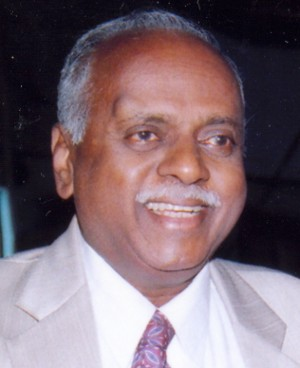
\includegraphics[scale=.6]{figures/authors/Prof_P_Venkataramaiah.jpg}} & 

\centerline{\large\bf Prof. P. Venkataramaiah}

\bigskip
Prof. P.Venkataramiah was a longtime colleague of Prof.G.Ramachandran in the Department of Physics, University of Mysore. He joined Yuvraja College, Mysore, in 1965, and moved over to Physics Department, Manasagangothri, Mysore, in1971. He obtained Ph.D. in 1978 from Mysore University. He was the Registrar of Mysore University during 1987-90. He later served with distinction as the Vice Chancellor of Kuvempu University from 1996 to 1999. He is currently the Chairman of Committee for the Development of Science in Schools (CDSS), University of Mysore. He leads a very active retired life and lives in Kuvempunagar, Mysuru.\\
&\\ 
\clineB{1-2}{2.5}
\end{tabular}



